\subsection{Base Software}
The base software is the foundation of every node. %NOT DONE AT ALL, THIS ALL WRONG

All slave nodes are customizable and modules can be swapped without flashing
the firmware. To implement this, module specific source code is executed in
its own thread. In the \texttt{Setup()} function, the module is determined
and the corresponding thread is started.

        \subsubsection{Determining the Module}

        \begin{figure}[H]
            \centering
            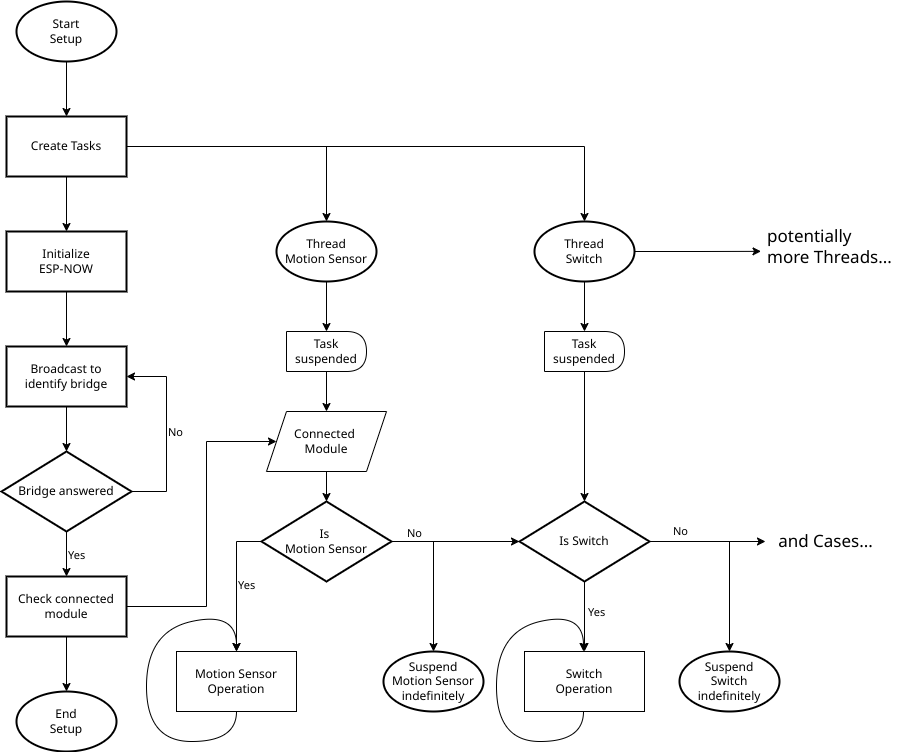
\includegraphics[width=0.95\textwidth]{./topics/flowcharts/Slave.drawio.png}
            \caption{Node Module Selection}
            \label{fig:NodeModuleSelection}
        \end{figure}
